% Add this to your preamble (at the top of your .tex file, before \begin{document}):
% \usepackage{subcaption}
% \usepackage{float}

\begin{frame}
\frametitle{Hàm số }
    \begin{tcolorbox}[colback=blue!10!, colframe=blue!50!black, title=Định nghĩa]
        \textit{Hàm} $f$ là một quy tắc cho tương ứng mỗi phần tử x thuộc tập hợp $X$ với một và chỉ một phần tử , kí hiệu $f(x)$, thuộc một tập hợp $Y$.
    \end{tcolorbox}
     \begin{figure}
      \centering
      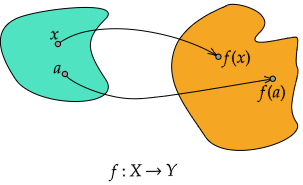
\includegraphics[width=6cm, height= 3cm]{Slides/figure/anhxa - Copy.png}
     \end{figure}
\end{frame}

\begin{frame}
\frametitle{Đồ thị hàm số}
   Đồ thị của \(f\) bao gồm mọi điểm \((x,y)\) sao cho \(y=f(x)\) với \(x\in X\).
  \begin{columns}
    \begin{column}{0.5\textwidth}
      \begin{figure}
        \centering
        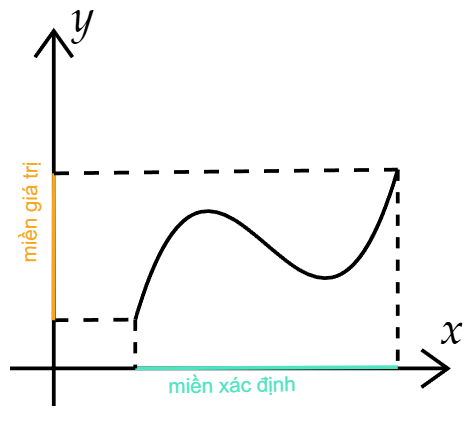
\includegraphics[width=5cm, height= 4cm]{Slides/figure/hamso1 - Copy.png}
      \end{figure}
    \end{column}
    \begin{column}{0.5\textwidth}
      Một số hàm số quen thuộc:
      \begin{itemize}
        \item \(y=\sin x : X= (-\infty, \infty), Y=[-1,1]\)
        \item \(y=\lvert x\rvert : X= (-\infty, \infty), Y=(0,\infty)\)
      \end{itemize}
      Chú ý, đây không phải là một hàm số:
    \begin{figure}
        \centering
        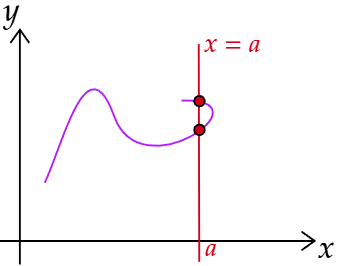
\includegraphics[width=4cm, height= 3cm]{Slides/figure/khongphaihamso - Copy.png}
      \end{figure}
    \end{column}
  \end{columns}
\end{frame}
    